\documentclass[12pt,letterpaper]{article}

\usepackage{common}
\usepackage{amsmath,amsfonts,amssymb,bbm}
\usepackage{palatino}
\usepackage[linkcolor=blue]{hyperref}
\usepackage{fullpage}
\usepackage{color}
\usepackage{enumitem}
\usepackage{titlesec}
\usepackage[textsize=tiny]{todonotes}
\usepackage{hyperref}
\hypersetup{
    colorlinks=true,
    linkcolor=blue,
    filecolor=magenta,
    urlcolor=cyan,
}

\newcommand{\TODO}[1]{\todo[inline]{#1}}
\newcommand{\R}{\mathbbm{R}}
\newcommand{\mba}{\mathbf{a}}
\newcommand{\mbb}{\mathbf{b}}
\newcommand{\boldphi}{\boldsymbol{\phi}}
\newcommand{\mbx}{\mathbf{x}}
\newcommand{\mbxt}{\tilde{\mathbf{x}}}
\newcommand{\Sigmat}{\tilde{\Sigma}}
\newcommand{\mbz}{\mathbf{z}}
\newcommand{\mbw}{\mathbf{w}}
\newcommand{\eps}{\epsilon}
\newcommand{\Ut}{\tilde{U}}
\newcommand{\angstrom}{\textup{\AA}}
\newcommand{\E}{\mathrm{E}}
\newcommand{\Var}{\mathrm{Var}}
\newcommand{\p}{\partial}

\newcommand{\false}{{\it false}}
\newcommand{\true}{{\it true}}
\newcommand{\nutr}{{\it nutr}}
\newcommand{\pois}{{\it pois}}


\begin{document}
\begin{center}
\LARGE{CS 181 Spring 2019 Section 2 Notes}\\
(Model Selection)
\end{center}

\section{Validation}

\subsection{Linear Regression}

Suppose we have data $\{(x_i, y_i)\}_{i=1}^n$, with $x_i, y_i\in \mathbb{R}$,
and we want to fit polynomial basis functions:
%
$$\boldphi(x)^\top = [\phi_1(x) = 1, \phi_2(x) = x, \ldots, \phi_{d+1}(x) = x^d]$$
$$h(\boldx; \boldw) = \boldw^\top\boldphi(x)$$
That is, we fit a degree $d$ polynomial. With a small dataset and too high of a $d$, we get overfitting. Obviously, this will generalize poorly to new data points. How can we solve this problem?

\subsection{Ridge Regression}

One solution to overfitting linear regression is through ridge regression, which minimizes a modified least squares loss function:
$$\mcL(D) = \sum_{i=1}^n (y_i - h(x_i; \boldw))^2 + \frac\lambda 2 ||\boldw||^2$$
Ridge regression is used to \emph{regularize} a model, making it simpler and allowing it to generalize better to new data. Indeed, the extra term penalizes overly large weights in $\boldw$, leading to smaller coefficients for a ``flatter'' polynomial:
\begin{center}
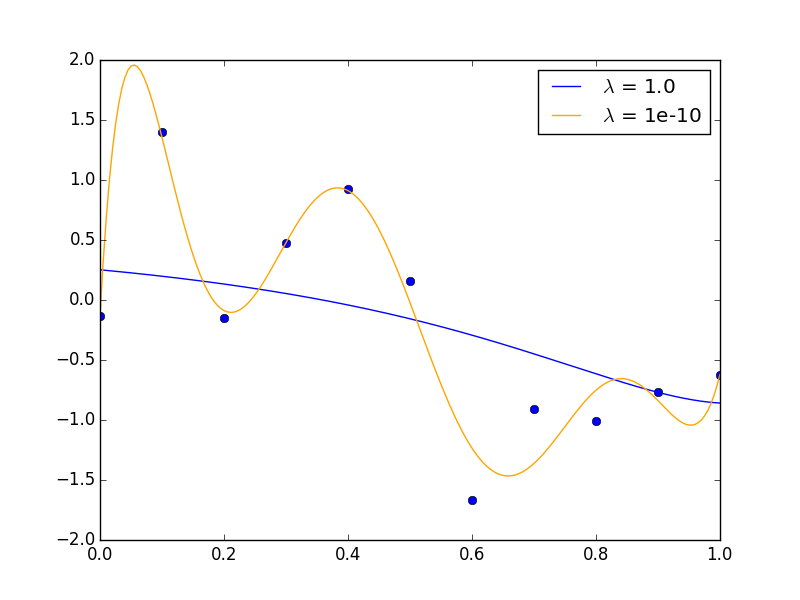
\includegraphics[scale=0.5]{regression}
\end{center}


\vspace{0.5cm}


\subsection{Validation Set: Model Selection}

We can do model selection through a \emph{validation set}, data that are separate from our training set used to fit the regression. By separating our full dataset into a training set and validation set (say in a 90/10 split), we can use our validation set to check our model's generalization ability on data it was not trained on. When tuning model parameters, we can train our models with different parameters on the training set and check their performance on the validation set in order to find the optimal value for the parameter.

\subsection{Cross Validation}

Cross validation is a more sophisticated technique for obtaining validation losses. Instead of splitting our data once into a 90/10 training/validation set, in $k$-fold cross validation, we split our data into $k$ equal chunks. For each chunk, we set it to be the validation set and use the rest of the data to fit our model. Then, we obtain a validation loss on our current chunk, and averaging over the 10 chunks gives the final validation loss. Cross validation can also be used to find optimal parameter values as described in the previous section - we simply have an improved way of computing validation losses by averaging. This reduces the variance in the resulting validation loss, as each example is used in estimating the validation loss.

See this \href{https://colab.research.google.com/drive/1hZcd_oV8o81y3jXCHp4xpfeDOJO76MPh}{notebook} for an interactive demo of how cross validation could be used.

\section{Bias-Variance Decomposition}

Bias-variance decomposition is a way of understanding how different sources of error (bias and variance) can affect the final performance of a model. A tradeoff between bias and variance is often made when selecting models to use, and can be informed by the results of the bias-variance decomposition.
\\ \\
\noindent \textbf{Exercise}: Decompose the generalization error into the sum of bias squared (systematic error), variance (sensitivity of prediction), and noise (irreducible error) by following the steps below (\textbf{try not to peek at your notes!}). You will find the following notation useful:
\begin{itemize}
  \item $h_D$: The trained model, $h_D: \mathcal{X} \mapsto \mathbb{R}$.
  \item $D$: The data, a random variable sampled $D\sim F^n$.
  \item $\boldx$: A new input.
  \item $y$: The true result of input $\boldx$. Conditioned on $\boldx$, $y$ is a r.v.
  (may be noise.)
  \item $\overline{y}$: The true conditional mean, $\overline{y}=\mathbb{E}_{y|\boldx}[y]$.
  \item $\overline{h}(\boldx)$: The prediction mean, $\overline{h}(\boldx)=\mathbb{E}_D[h_D(\boldx)]$.
\end{itemize}
\begin{enumerate}
    \item Start with the equation for the generalization error - the expected error, in least squares terms, on an unseen sample:
    \begin{align}
        \mathbb{E}_{D, \, y|\boldx}[(y-h_D(\boldx))^2]\notag
    \end{align}
    and use the linearity of expectation to derive an equation of the form:
    \begin{align}
        \underbrace{\mathbb{E}_{y|\boldx}[(y-\overline{y})^2]}_\text{noise}
+\underbrace{\mathbb{E}_D[(\overline{y}-h_D(\boldx))^2]}_\text{bias+var}
+ *******
    \end{align}{}
    where the *s denote a third term. What is this third term? (\textbf{Hint}: add and subtract $\overline{y}$).
    \item
    Show that this third term is equal to 0 (\textbf{Hint}: take advantage of the fact that $\overline{y}$ and $h_D(\boldx)$ do not depend on $y|x$.
    \item
    The first term in~(1) is the noise. We therefore want to decompose the second term into the bias and variance. Again, using the linearity of expectation, re-write the second term in equation~(1) in the form:
    \begin{align}
        \underbrace{(\overline{y}-\overline{h}(\boldx))^2}_\text{bias squared}+\underbrace{\mathbb{E}_D[(\overline{h}(\boldx)-h_D(\boldx))^2]}_\text{variance}
+2\mathbb{E}_D[(\overline{y}-\overline{h}(\boldx))(\overline{h}(\boldx)-h_D(\boldx))]
    \end{align}
    show that the third term is equal to 0.
    \item
    Plug the results of part 3 back into~(1) to show that we have decomposed the error into noise, bias, and variance.

\newpage

\end{enumerate}
% \noindent \textbf{Solution}:
% \begin{enumerate}
%     \item Follow the hint: \begin{align*}
%   & \mathbb{E}_{D, \, y|\boldx}[(y-h_D(\boldx))^2]\notag \\
%   &= \mathbb{E}_{D, \, y|\boldx}[(y-\overline{y}+\overline{y}-h_D(\boldx))^2]\notag  \\
%  &=\underbrace{\mathbb{E}_{y|\boldx}[(y-\overline{y})^2]}_\text{noise}
% +\underbrace{\mathbb{E}_D[(\overline{y}-h_D(\boldx))^2]}_\text{bias+var}
% +\underbrace{2\mathbb{E}_{D, \, y|\boldx}[(y-\overline{y})(\overline{y}-h_D(\boldx))]}_\text{0}
% \end{align*}
% \item Using the hint:
% $$
% 2\mathbb{E}_D[\overline{y}-h_D(\boldx)
% \cdot \mathbb{E}_{y|\boldx}[y-\overline{y}]]
%   = 2\mathbb{E}_D[\overline{y}-h_D(\boldx)
% \cdot 0] = 0.$$
% \item
% Following a similar procedure as in part 1:
% \begin{align*}
%  & \mathbb{E}_D[(\overline{y}-h_D(\boldx))^2]\notag \\
%  &= \mathbb{E}_D[(\overline{y}-\overline{h}(\boldx)+\overline{h}(\boldx)-h_D(\boldx))^2] \notag \\
%  &= \underbrace{(\overline{y}-\overline{h}(\boldx))^2}_\text{bias squared}+\underbrace{\mathbb{E}_D[(\overline{h}(\boldx)-h_D(\boldx))^2]}_\text{variance}
% +\underbrace{2\mathbb{E}_D[(\overline{y}-\overline{h}(\boldx))(\overline{h}(\boldx)-h_D(\boldx))]}_\text{0}
% \end{align*}
% where the third term is 0 by:
% $$
% 2(\overline{y}-\overline{h}(\boldx))
% \mathbb{E}_D[\overline{h}(\boldx)-h_D(\boldx)]
% = 2(\overline{y}-\overline{h}(\boldx))(0) = 0.
% $$
% \item
% Substituting~(2) back into~(1), we have:
% %
% \begin{align*}
% &  \mathbb{E}_{D, \, y|\boldx}[(y-h_D(\boldx))^2] \\
% &= \mathbb{E}_{y|\boldx}[(y-\overline{y})^2]+
% (\overline{y}-\overline{h}(\boldx))^2
% +
% \mathbb{E}_D[(\overline{h}(\boldx)-h_D(\boldx))^2]
% \\
% &=\mbox{noise}(\boldx)+(\bias(h(\boldx)))^2
% +\var_D(h_D(\boldx)).
% \end{align*}
% Considering the expectation over $\boldx$ (you are not asked to do this in the exercises), the
% generalization error is:
% %
% \begin{align*}
% \mathbb{E}_{\boldx}\left[\mbox{noise}(\boldx)+
% (\bias(h(\boldx)))^2
%     +\var_D(h_D(\boldx))\right]
%   \end{align*}
% \end{enumerate}

\subsection{Limitations}
Although the bias-variance decomposition provides some interesting insights into model selection from a complexity perspective, it has limited practical value, as it is based on averages of independent data sets drawn from some distribution. In practice, however, we only have a single observed data set.
The bias and variance can be estimated through ``bootstrap'' style
approaches where we sample with replacement to form additional
data sets, but still--- why not more directly compute validation loss
and use this to find the best model? The main interest in the bias-variance decomposition is to gain conceptual insight.

\section{Ensemble Methods}
Ensemble methods take advantage of multiple models to obtain better predictive accuracy than with a single model alone. The two most common types of ensemble methods are bagging and boosting.

\subsection{Bootstrap aggregating (Bagging)}
In bagging, we fit each individual model on a random sample of the training set. To predict data in the test set, we either use an average of the predictions from the individual models (for regression) or take the majority vote (for classification). As an average of models, bagging tends to decrease the variance of a learning algorithm without changing the bias. An example is a random forest, which trains multiple decision trees and takes the average prediction from the ensemble of learned models.

\subsection{Boosting}

In boosting, we train the individual models sequentially. Thus, after training the $i^{th}$ model on a sample of the training set, we train the $(i+1)^{th}$ model on a new sample based on the performance of the $i^{th}$ model. Examples classified incorrectly in the previous step receive higher weights in the new sample, encouraging the new model to focus on those examples. During testing, we take a weighted average or weighted majority vote of the models' predictions based on their respective training accuracies on their reweighted training data (i.e. higher models have larger weights). A common example is the Adaboost algorithm.

\newpage

\section{Practice Questions}

\begin{enumerate}

\item {\bf Ridge Regression }\\
\fbox{\parbox{\linewidth}{%
Suppose we have some data matrix $\boldX \in \mathbb{R}^{n \times m}$ and targets $\boldy \in \mathbb{R}^n$. Suppose the data are orthogonal*, i.e. satisfies $\boldX^\top \boldX = \boldI$. Show that if $\widehat{\boldw}$ is the solution to linear regression, and $\widehat{\boldw}_{ridge}$ is the solution to ridge regression, then
$$\widehat{\boldw}_{ridge} = \frac{1}{1 + \lambda} \widehat{\boldw}$$
This explicitly illustrates the phenomenon of weight shrinkage.\\
}}\let\thefootnote\relax\footnote{* Orthogonal data is a very special case in which the inner product between any two distinct features is zero. Normally we expect features to be correlated. But it is used to gain this clean illustration of the effect of ridge regression. Technically, we have $\boldX = [\boldv_1, \ldots, \boldv_m]$ where $\boldv_1, \ldots, \boldv_m$ are $n$ dimensional, orthogonal column vectors.}

\vspace{\baselineskip}

% Solution

% Recall that the linear regression solution is
% $$\widehat{\boldw} = (\boldX^\top \boldX)^{-1} \boldX^\top \boldy$$
% and recall from homework that the ridge regression solution is
% $$\widehat{\boldw}_{ridge} = (\boldX^\top \boldX + \lambda \boldI)^{-1} \boldX^\top \boldy$$
% If $\boldX^\top\boldX = \boldI$, we see that
% \begin{align*}
% \widehat{\boldw} = \boldX^\top \boldy \\
% \widehat{\boldw}_{ridge} = \frac{1}{1 + \lambda} \boldX^\top \boldy \\
% \end{align*}
% hence giving us the result.

\newpage

\item {\bf Bias and Variance}\\
\fbox{\parbox{\linewidth}{%
We consider a very simple example where the data is a univariate Gaussian, with $x_i \sim \mcN(\mu,1)$ with known variance but unknown mean. In this case, there are no features, and the hypothesis doesn't depend on $x$. A very simple hypothesis, for example, is the sample mean
$$h_D= \overline{x} = \frac 1n \sum_{i=1}^n x_i$$
for data $(x_1,\ldots,x_n)\in \mathbb{R}^n$.  Calculate the bias and variance for the following two hypotheses:
\begin{enumerate}
\item Estimate 1: Use the same mean of data $D$.
\item Estimate 2: Use the constant hypothesis, 0.
\end{enumerate}
}}

\vspace{\baselineskip}

% Solution

% \begin{enumerate}
% % \item The bias equals $0$, as $D$ has the exact distribution as the true distribution. The variance of our prediction is the same as the variance of $D = 1$.
% \item The bias is $\mu - E_D[\overline{x}] = \mu - E_D[(1/n)\sum x_i]=0$. The variance is $E_D[(\overline{x} - \mu)^2] = \sigma^2 / n$, the variance of the sample mean on $n$ examples (as is standard).

% \item The bias equals $\mu$, the expected difference between the estimator and the true value. This prediction is constant, so the variance of our prediction is $0$.
% \end{enumerate}

\newpage

\item {\bf Deriving Lasso Regularization with Lagrange Multipliers }\\
\fbox{\parbox{\linewidth}{%
Show that minimization of the unregularized sum-of-squares error function given by
\begin{align*}
E_D(\boldw) = \frac{1}{2}\sum_{n = 1}^N (t_n - \boldw^\trans \phi(\boldx_n) )^2,
\end{align*}
subject to the constraint
\begin{align*}
\sum_{j = 1}^M |w_j| \leq \eta ,
\end{align*}
is equivalent to minimizing the regularized error function
\begin{align*}
\frac{1}{2} \sum_{n = 1}^N (t_n - \boldw^\trans \phi(\boldx_n) )^2 + \frac{\lambda}{2} \sum_{j = 1}^M |w_j|
\end{align*}
}}

\vspace{\baselineskip}

% Solution

% Rewrite the constraint as
% \begin{align*}
% \sum_{j = 1}^M |w_j| - \eta \leq 0
% \end{align*}

% We get the Lagrangain function
% \begin{align*}
% L(\boldw, \lambda) = \frac{1}{2} \sum_{n = 1}^N (t_n - \boldw^\trans \phi(\boldx_n) )^2 + \frac{\lambda}{2} \sum_{j = 1}^M (|w_j| - \eta)
% \end{align*}

% where we introduce the factor of $1/2$ in front of the second term for convenience. We see immediately that the above function is equal to the regularized error function plus the terms of $\eta$ which do not depend on $\boldw$. Therefore, minimizing the Lagrangian with respect to $\boldw$ will give the same $\boldw^*$ as minimizing the regularized error function.

\newpage

\item {\bf Priors for Model Selection }\\
\fbox{\parbox{\linewidth}{%
Suppose you had three models, $M_1, M_2, M_3$, each increasing in complexity. For example, you could imagine that the models represented unregularized polynomial regression, with $M_1$ linear regression, $M_2$ quadratic regression, and $M_3$ cubic regression. Within the context of Bayesian model selection, come up with a way to penalize the complexity of a model so you do not always choose $M_3$. Additionally, explain why, in many cases, Bayesian model selection will recover the simplest model to explain the data without explicit penalization.
}}

\vspace{\baselineskip}

% % Solution

% Choose the prior over the model space to assign higher probability to the simpler models. This is the same thing that we did to encourage less complex parameters in Bayesian linear regression; we put a prior over the weight vector assigning the highest probability to weight vectors that lie close to zero. This is a a phenomenon known as Bayesian Occam's Razor and is discussed on in Bishop (pg. 164, fig. 3.13). Briefly, since simpler models can explain a smaller subset of data than more complex models, and each model has to integrate to 1, the simpler models can put higher probabilities on the data that they do describe than the complex models, which must put some of their mass on the data that the simpler model cannot describe.

\end{enumerate}

\end{document}
